\documentclass{beamer}
\input{themes/packages.tex}
\usetheme{apertus}

\title{Introduction to JTAG} 
\titlegraphic{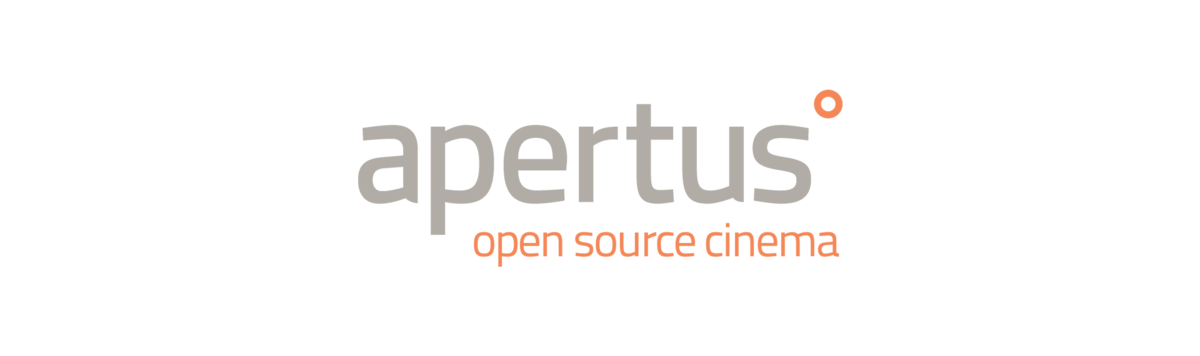
\includegraphics[width=10cm]{images/apertus_logo.png}}
\author{Swaraj Hota}
\date

\begin{document}
{
    \setbeamertemplate{footline}{} 
    \frame{\titlepage}
}

\section*{Contents}

\begin{frame}{Contents}
    \tableofcontents
\end{frame}

\subsection{Boundary Scan}

\begin{frame}{What is Boundary Scan?}
    \begin{itemize}
    \item Allows you to debug individual IO pins of a chip in an assembled PCB
        (without physical access)
    \item Uses extra circuitary (called \textit{wrapper}), one ``test cell" attached to each pin
    \item These test cells provide a way to capture/update data
    \item All test cells are ``daisy chained" (think a single big shift register)
    \item We essentially need a serial data i/p pin and an o/p pin to shift-in 
            and shift-out bits from all the pins
    \item The \emph{wrapper} lies dormant (invisible) during normal operation 
    \end{itemize}
\end{frame}

\subsection{JTAG Intro}

\begin{frame}{Enter... JTAG!}
    \begin{itemize}
    \item JTAG, the IEEE 1149.1 standard, was formalized
    \item Also called the \emph{boundary scan standard} 
    \item A standardized way to do \emph{boundary scan}
    \end{itemize}
\end{frame}

\begin{frame}{So... JTAG is just for Boundary Scan?}
    \begin{itemize}
    \item Originally that was its purpose, but it turned out to be much more versatile!
    \item Not just single chips, any number of chips can be debugged in a board
        (again, daisy chained)
    \item And not just the ``boundary", interal system logic can also be debugged
    \item Further, can also be used for programming chips! (like FPGAs)
    \end{itemize}
\end{frame}

\subsection{JTAG Architecture}

\begin{frame}{Schematic of a JTAG enabled device}
    \includegraphics[width=7cm]{images/schematic_diagram_jtag_enab.jpg}
\end{frame}

\begin{frame}{Test Access Port (TAP)}
The JTAG port or Test Access Port (TAP) requires only 5 pins:
    \begin{itemize}
    \item TDI: Test Data Input (Serial Data in) 
    \item TDO: Test Data Output (Serial Data out)
    \item TCK: Test Clock
    \item TMS: Test Mode Select (Change states in JTAG state machine)
    \item TRST: Test Reset (Optional, to reset JTAG state machine)
    \end{itemize}
\end{frame}

\begin{frame}{JTAG Registers}
    \begin{itemize}
    \item Standard specifies one Instruction Register (IR) and various 
        Data Registers (DR) to select from
    \item Mandatory Data registers:
        \begin{itemize}
        \item Boundary Scan Register (BSR) - the \emph{wrapper}
        \item Bypass Register (BYPASS) - one bit register
        \end{itemize}
    \item Optional Data Registers:
        \begin{itemize}
        \item Device ID Register (IDCODE)
        \item Various Device specific registers
        \end{itemize}
    \item The register which is selected will shift-in bits from TDI and shift-out
        bits from TDO
    \end{itemize}
\end{frame}

\begin{frame}{TAP Controller}
    \begin{itemize}
    \item Contains the \emph{JTAG/TAP State Machine}
    \item Also the Instruction Register and Instruction Decoder
    \item According to the current state in the state machine, one of the data 
        register or instruction register will be selected/scanned/captured/updated
    \item Which data register is selected will depend on the instruction passed
    \end{itemize}
\end{frame}

\begin{frame}{TAP State Machine}
    \includegraphics[width=6cm]{images/tap_state_machine.jpg}
\end{frame}

\begin{frame}{JTAG Instructions}
    \begin{itemize}
    \item Mandatory instructions:
        \begin{itemize}
        \item BYPASS (111...) - Use BYPASS Register (Passthrough)
        \item EXTEST (000...) - Use BSR (Capture-DR -> Shift-DR -> Update-DR)
        \item SAMPLE/PRELOAD - Use BSR (when device in normal mode)
        \end{itemize}
    \item Optional instructions:
        \begin{itemize}
        \item IDCODE - Use IDCODE register 
        \item INTEST - Use BSR (test internal core-logic)
        \item Various other design specific instructions
        \end{itemize}
    \end{itemize}
\end{frame}

\end{document}
